\documentclass[10pt]{article}
\usepackage{graphicx} % Required for inserting images
\usepackage{natbib}
\usepackage{geometry}
\usepackage{multicol}

\geometry{a4paper, left = 20mm, right = 10mm}

\title{TRES Workshop}
\author{Thijs Janzen}
\date{17th January 2024}


\begin{document}

\maketitle

\newpage

\section*{Abstract}
{\tiny small text}\\
{\Huge large text}

\section{Introduction}
% \begin{multicols}{2}
We can \textit{italicize} text or make text \textbf{bold}. Or \textit{ \textbf{both} }. \newline
This is another text. \\
On another line.\\
In section \ref{sec:methods} we explain what we do.
% \end{multicols}

\section{Methods}\label{sec:methods}

\section*{Math}

The frequency of allele X is given by $p = 1 - q$. And not by $\pi$ or $\lambda$ or $\tau$.

\begin{equation}
Hw = p^2 + 2pq + q^2
\label{eq:hw}
\end{equation}

\begin{equation}
A = \frac{1}{n} \sum_{i=1}^n x_i
\label{eq:mean}
\end{equation}

\begin{equation}
P_i^2 = 5
\label{eq:1}
\end{equation}

\section{Results}
\subsection{Figures}

In Fig. \ref{fig:linneausborg} we show a picture of the building in which this workshop was given. In the workshop, we dealt with equation \ref{eq:hw} on Hardy-Weinberg and equation \ref{eq:mean} on calculating the mean.
% comments are started with %%

\begin{figure}[ht]
    \centering
    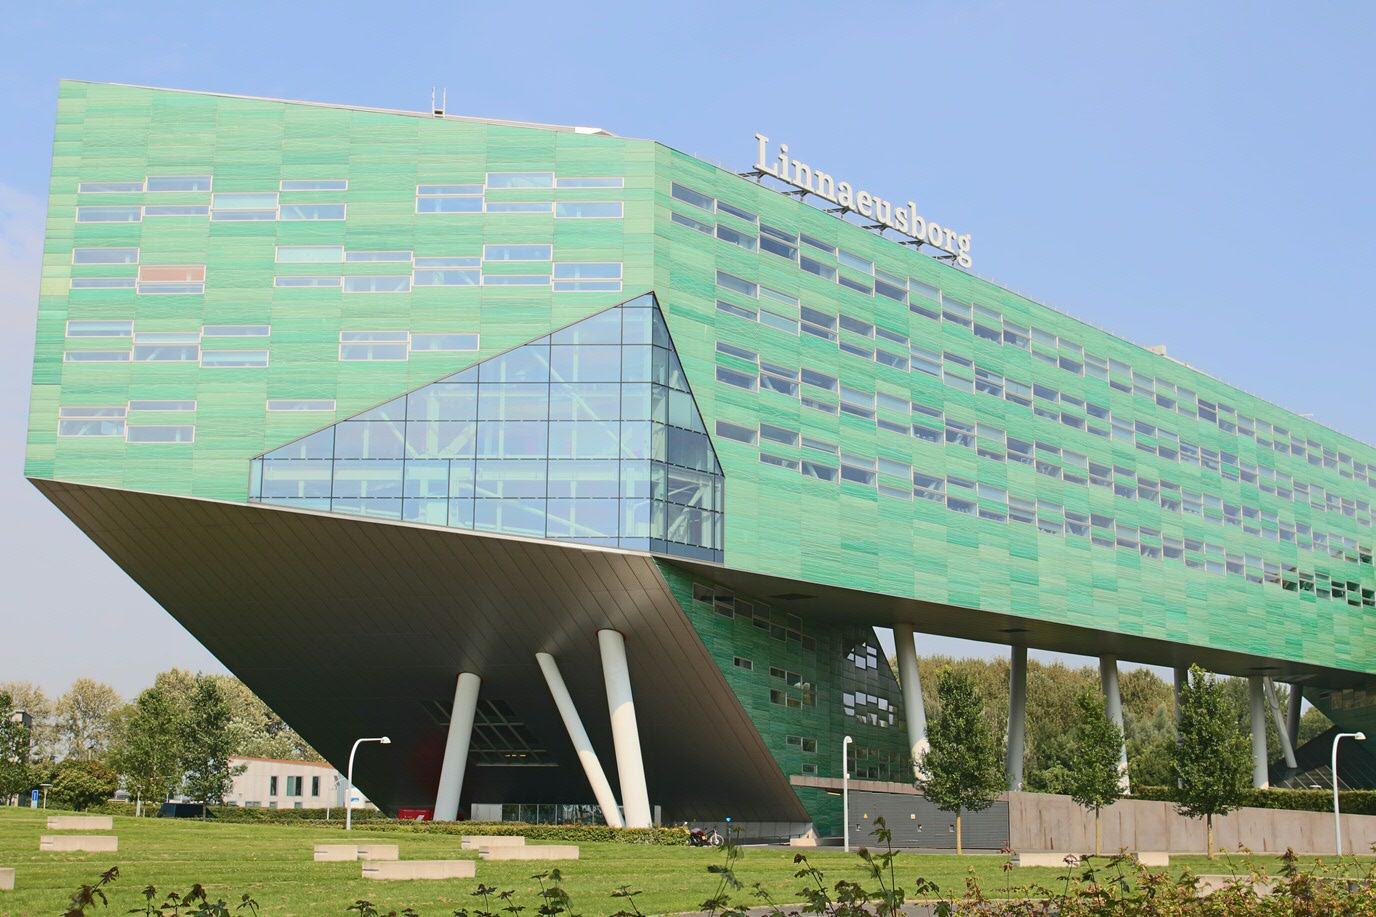
\includegraphics[width = 0.3\textwidth]{linnaeusborg1.jpg}
    \caption{This is the Linneausborg}
    \label{fig:linneausborg}
\end{figure}

\subsection{Tables}
\begin{table}[ht]
    \centering
    \begin{tabular}{|l|c|r|}
    \hline
    \textbf{Country}  & \textit{Food} & \textbf{\textit{Continent}} \\
     \hline
     Netherlands  & Kroket & Europe \\
     Mexico & Tacos & America \\
     Thailand & Pad Thai & Asia \\
     \hline
    \end{tabular}
    \caption{Food types across the world}
    \label{tab:food}
\end{table}

\section{Discussion}
Evolvability \citep{riederer2022} is often discussed by \cite{riederer2022}.



\bibliographystyle{apalike}

\bibliography{library.bib}

\end{document}
